\documentclass[12pt]{article}
\usepackage{amsmath}
\usepackage{gensymb}
\usepackage{float}
\usepackage{graphicx}
\usepackage{graphics}
\graphicspath{{storage/self/primary/Download/assignment/fig}}
\graphicspath{{storage/self/primary/Download/assignment/table}}
\let\vec\mathbf
\providecommand{\abs}[1]{\ensuremath{\left|#1\right|}}
\providecommand{\brak}[1]{\ensuremath{\left(#1\right)}}
\begin{document}
\title{\textbf{ASSIGNMENT 2}}
\date{}
\maketitle
\textbf{Question :} Two lines passing through the point(2,3) intersect each other at an angle of $60\degree$.If slope of one line is 2,find equation of the other line.


\textbf{Solution :}
\begin{table}[H]
    \centering
       \begin{tabular}{|c|c|c|}
    \hline
    \textbf{Input Parameters} &\textbf{Description} &\textbf{Value} \\
    \hline
     $\vec{O}$& Center(at origin)&$\vec{0}$\\
     \hline
 $r$ & Radius &1\\
 \hline
 $\theta$&-&$100\degree$\\
 \hline
 $\alpha$&-&$165.4\degree$\\
 \hline
 $\beta$&-&$5\degree$\\
 \hline
  \end{tabular}

   \caption{Table of input parameters}
    \label{tab:tab:1}
\end{table}
\begin{table}[H]
    \centering
    \begin{tabular}{|c|c|c|}
    \hline
        \textbf{Output Parameters} &\textbf{Description} &\textbf{Value} \\
\hline
          $\vec{Q}$ & Point &$\myvec{\cos{\theta_1}\\\sin{\theta_1}}$\\
          \hline
          $\vec{P}$ & Point &$\myvec{\cos{\theta_2}\\\sin{\theta_2}}$ \\
         \hline
          $\vec{R}$ & Point &$\myvec{\cos{\theta_3}\\sin{\theta_3}}$ \\
         \hline
    \end{tabular}


    \caption{Table of output parameters}
    \label{tab:tab:2}
\end{table}
So,
\begin{align}
    \tan{60\degree}=\sqrt{3}&=\abs{\frac{2-m_2}{1+2m_2}}\\
\implies m_2&=\frac{2-\sqrt{3}}{2\sqrt{3}+1}\\
or,&=-\frac{\brak{2+\sqrt{3}}}{2\sqrt{3}-1}
\end{align}
So,the equation of the line is
\begin{align}
\brak{y-3}&=\frac{2-\sqrt{3}}{2\sqrt{3}+1}\brak{x-2}\\
or,\brak{y-3}&=-\frac{\brak{2+\sqrt{3}}}{2\sqrt{3}-1}\brak{x-2}
\end{align}

\textbf{Figure :}                               
\begin{figure}[H]                            
	\centering                        
	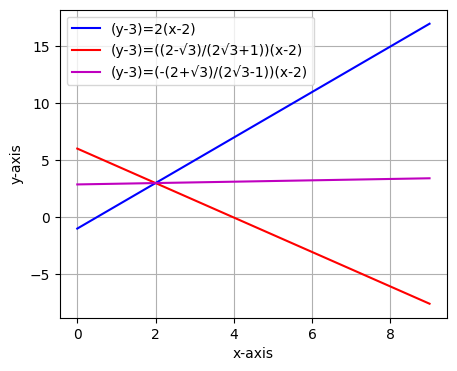
\includegraphics[width=\columnwidth]{fig/asgnt.png}                          
	\caption{Required Figure}
	\label{fig:fig:1}
\end{figure}
\end{document}

